\subsection{Synonym discrimination}
\label{sec:synonym}

Next we simulate the task of distinguishing between pairs of synonyms, i.e.\ words with different acoustic forms but the same meaning. With a representation encoding phonological form, our expectation is that the task would be easy; in contrast, with a representation which is invariant to phonological form in order to encode meaning, the task would be hard. 

We generate a list of synonyms for each noun, verb and adjective in the validation data using Wordnet \citep{miller1995wordnet} synset membership as a criterion. Out of these generated word pairs, we select synonyms for the experiment based on the following criteria:
\begin{itemize}
\item both forms clearly are synonyms in the sense that one word can be replaced by the other without changing the meaning of a sentence,
\item both forms appear more than 20 times in the validation data, 
\item the words differ clearly in form (i.e. they are not simply variant spellings like {\it donut/doughnut, grey/gray}),
\item the more frequent form constitutes less than 95\% of the occurrences.
\end{itemize}
This gives us 2 verb, 2 adjective and 21 noun pairs.

For each synonym pair, we select the sentences in the validation set in which one of the two forms appears. We use the POS-tagging feature of NLTK \citep{bird2006nltk} to ensure that only those sentences are selected in which the word appears in the correct word category (e.g.\ {\it play} and {\it show} are synonyms when used as nouns, but not when used as verbs). We then generate spoken utterances in which the original word is replaced by its synonym, resulting in the same amount of utterances for both words of each synonym pair.

\begin{figure}[!ht]
  \centering
  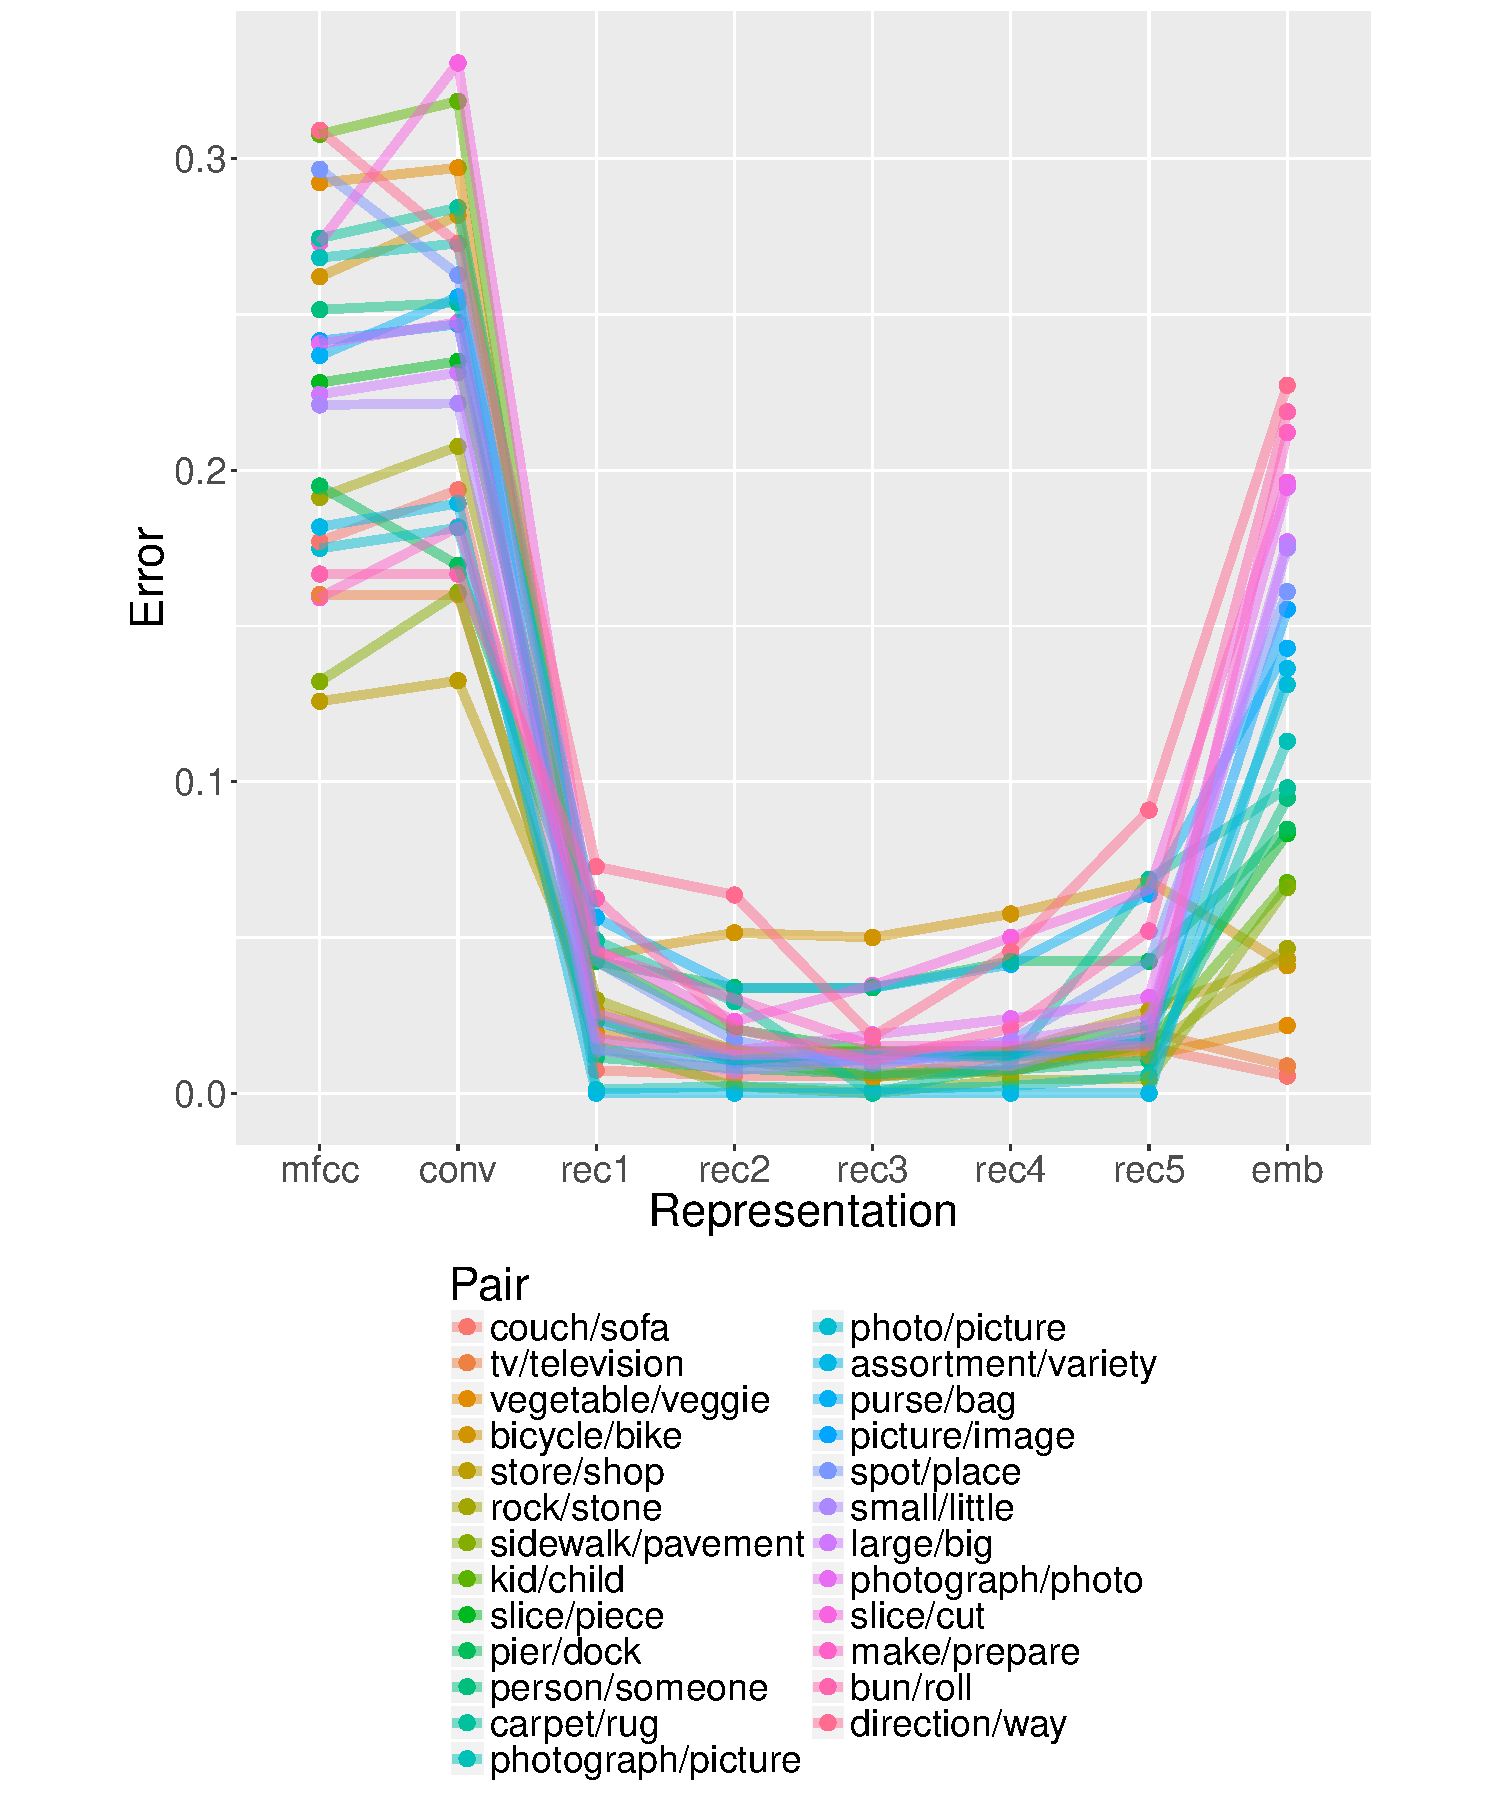
\includegraphics[scale=0.3]{figures/synonym.pdf}
  \caption{Synonym discrimination error rates, per representation and synonym pair.}
  \label{fig:synonyms}
\end{figure}


For each pair we generate a binary classification task using the MFCC features, the average activations in the convolutional layer, the average unit activations per recurrent layer, and the sentence embeddings as input features. For every type of input, we run 10-fold cross validation using Logistic Regression to predict which of the two words the utterance contains.  We used an average of 672 (minimum 96; maximum 2282) utterances for training the classifiers.

Figure~\ref{fig:synonyms} shows the error rate in this classification task for each layer and each synonym pair. Recurrent layer activations are more informative for this task than MFCC features or activations of the convolutional layer.  Across all the recurrent layers the error rate is small, showing that some form of phonological information is present throughout this part of the model. However, sentence embeddings give relatively high error rates suggesting that the attention layer acts to focus on semantic information and to filter out much of phonological form.

